%%%%%%%% ICML 2026 SUBMISSION %%%%%%%%%%%%%%%%%
% Correlated Thompson Sampling via LLM-Derived Covariance Structure
% for Combinatorial Semi-Bandits

\documentclass{article}

\usepackage{microtype}
\usepackage{graphicx}
\usepackage{subcaption}
\usepackage{booktabs}
\usepackage{hyperref}
\newcommand{\theHalgorithm}{\arabic{algorithm}}

\usepackage{icml2026}

\usepackage{amsmath}
\usepackage{amssymb}
\usepackage{mathtools}
\usepackage{amsthm}
\usepackage{algorithm}
\usepackage{algorithmic}
\usepackage{xcolor}
\usepackage{multirow}

\usepackage[capitalize,noabbrev]{cleveref}

\theoremstyle{plain}
\newtheorem{theorem}{Theorem}[section]
\newtheorem{proposition}[theorem]{Proposition}
\newtheorem{lemma}[theorem]{Lemma}
\newtheorem{corollary}[theorem]{Corollary}
\theoremstyle{definition}
\newtheorem{definition}[theorem]{Definition}
\newtheorem{assumption}[theorem]{Assumption}
\theoremstyle{remark}
\newtheorem{remark}[theorem]{Remark}

\newcommand{\R}{\mathbb{R}}
\newcommand{\E}{\mathbb{E}}
\newcommand{\Prob}{\mathbb{P}}
\newcommand{\opt}{S^{\star}}
\newcommand{\gap}{\Delta_{\min}}
\newcommand{\CorrCTS}{\textsc{CorrCTS}}
\newcommand{\CorrFull}{\textsc{CorrCTS-Full}}
\newcommand{\RobustCorr}{\textsc{RobustCorrCTS}}
\newcommand{\EdgePrune}{\textsc{CorrCTS-Prune}}
\newcommand{\KMRefine}{\textsc{CorrCTS-KM}}

\icmltitlerunning{Correlated Thompson Sampling via LLM-Derived Covariance for Combinatorial Semi-Bandits}

\begin{document}

\twocolumn[
  \icmltitle{Correlated Thompson Sampling via LLM-Derived\\Covariance Structure for Combinatorial Semi-Bandits}

  \icmlsetsymbol{equal}{*}

  \begin{icmlauthorlist}
    \icmlauthor{Anonymous Author(s)}{anon}
  \end{icmlauthorlist}

  \icmlaffiliation{anon}{Anonymous Institution}

  \icmlcorrespondingauthor{Anonymous Author(s)}{anonymous@example.com}

  \icmlkeywords{combinatorial bandits, Thompson sampling, large language models, correlated sampling}

  \vskip 0.3in
]

\printAffiliationsAndNotice{}

% ===========================================================================
% ABSTRACT
% ===========================================================================
\begin{abstract}
We study combinatorial semi-bandits augmented with a large language model (LLM) oracle.
Existing methods inject LLM output directly into the posterior as priors, pseudo-observations, or arm recommendations.
We show that this belief-injection approach is fragile because LLM accuracy depends on the estimates it receives as input: in one configuration, the same LLM achieves 4/5 top-$m$ accuracy when warm-started with Thompson sampling estimates and 0/5 with round-robin estimates.
We propose using the LLM for \emph{correlation structure} instead.
A single cluster query is converted to a positive-definite covariance matrix via an RBF kernel over cluster ranks; only the sampling step changes, and the Beta posteriors are updated from real rewards alone.
On synthetic Bernoulli instances ($T{=}2{,}500$, $n{=}320$), \CorrFull{} reduces regret by 18.9\% versus CTS ($p < 0.0001$, Holm-Bonferroni), of which 12.7 points are attributable to LLM cluster quality via a random-cluster ablation.
On a synthetic categorical recommendation benchmark with planted latent category structure ($d{=}200$, $m{=}5$), the reduction reaches 33.8\% with a 135/0 win/loss ratio, while warm-start CTS offers no benefit.
This benchmark tests whether the kernel exploits latent cluster structure when present; it does not test whether the LLM discovers structure in real click logs.
\end{abstract}

% ===========================================================================
% 1. INTRODUCTION
% ===========================================================================
\section{Introduction}\label{sec:intro}

We study the stochastic combinatorial semi-bandit problem.
A learner selects $m$ arms from a ground set of $d$ arms each round, observes a Bernoulli reward for each selected arm, and minimizes cumulative regret over $T$ rounds.
Combinatorial Thompson Sampling (CTS) \citep{wang2018cts} maintains independent Beta posteriors and samples each arm's mean independently.
This ignores any structure among arms, even when structure is readily available.

A natural source of structural information is a large language model.
Existing LLM-augmented bandit methods inject the LLM's output as a \emph{belief}: \citet{krishnamurthy2024canllms} study in-context exploration; \citet{alamdari2024jumpstarting,bayley2025jumpstart} warm-start bandits with LLM-generated priors; \citet{sun2025tsllm} mix LLM arm recommendations with Thompson sampling.
In each case, the LLM's output enters the posterior as a prior shift, a pseudo-observation, or a direct arm recommendation.
A separate line, \citet{cao2026libra}, uses LLM guidance in bandit recourse for personalized treatment planning and is orthogonal to our setting.

Belief injection is fragile, and we trace the fragility to a specific phenomenon that existing models do not capture: the LLM's answer quality depends on the estimates it receives as input.
In a representative configuration ($d=25$, $m=5$, 20 seeds), GPT-5.4 achieves 4 out of 5 top-$m$ accuracy after 30 rounds of CTS warmup, which concentrates pulls on promising arms, and 0 out of 5 after 30 rounds of round-robin, which spreads pulls uniformly.
Same model, same prompt template, same horizon; only the input estimates differ.
This single-configuration diagnostic is illustrative, not conclusive; replication across $(d, m)$ settings and warmup strategies is forthcoming in the camera-ready.
Oracle quality is therefore endogenous to the bandit's learning trajectory.
When $\hat\mu$ is noisy, belief injection amplifies errors; when $\hat\mu$ is accurate, the LLM's information is redundant.
The window in which belief injection helps is narrow, and existing theoretical models for LLM-bandits that treat oracle quality as an exogenous parameter $\epsilon$ \citep{sun2025tsllm} do not reach inside this window.

We propose a different design: use the LLM for \emph{structure}, not \emph{belief}.
We ask the LLM which arms behave similarly and obtain a partition into clusters.
When we sample posterior values, we draw \emph{correlated} samples for same-cluster arms rather than independent ones.
Observing arm 3's reward now implicitly informs our sampling of arms 7 and 12 whenever the LLM has placed them in the same cluster.
The correlation matrix is an RBF kernel over a cluster-rank embedding, which is positive definite by construction (\Cref{prop:pd}).
The Beta posteriors are never touched by the LLM; only the sampling step changes.
When the LLM is wrong, bad off-diagonal entries add noise to the samples; the diagonal and the posterior means remain uncontaminated, and performance degrades gracefully to CTS.

Our contributions are the following.
We design \CorrFull{}, a correlated Thompson sampling algorithm built from a single LLM cluster query.
On 16 synthetic configurations ($n{=}320$ paired trials, $T{=}2{,}500$), \CorrFull{} reduces regret by 18.9\% versus CTS ($p < 0.0001$, Holm-Bonferroni corrected).
A random-cluster ablation isolates 12.7 percentage points of this gain to LLM cluster quality, and a block-diagonal variant does not beat random clusters, showing that the inter-cluster structure captured by the RBF kernel drives the improvement.
We develop two data-adaptive variants, \EdgePrune{} and \KMRefine{}, that refresh the covariance from observed data and sustain a 6.1--6.8\% advantage at $T{=}25{,}000$ ($n{=}480$), validated on held-out configurations.
On a synthetic categorical recommendation benchmark with planted category structure (MIND-style, $d{=}200$, $m{=}5$), the reduction reaches 33.8\% with a 135/0 win/loss ratio against CTS; warm-start CTS, the belief-injection baseline, provides no benefit on this task.

% ===========================================================================
% 2. RELATED WORK
% ===========================================================================
\section{Related Work}\label{sec:related}

\textbf{Combinatorial semi-bandits.}
\citet{chen2013cucb} introduced the CMAB framework with CUCB, achieving $O(d \log T / \gap)$ regret.
\citet{kveton2015tight} proved tight $O(d \log T / \gap)$ bounds for the semi-bandit setting.
\citet{combes2015combinatorial} proposed ESCB, the canonical structured-combinatorial baseline: given a linear feature matrix $X \in \R^{d \times p}$ with $\mu = X\theta$, ESCB maintains a confidence ellipsoid on $\theta$ and selects actions by a concentration index, achieving an $\sqrt{m}$ improvement in the dependence on $m$.
Our LLM oracle returns a partition rather than a feature matrix that ESCB consumes directly; a one-hot cluster-indicator extension is feasible but imposes a rigid within-cluster homogeneity assumption that our RBF construction explicitly relaxes, so we treat ESCB as out of scope for the head-to-head comparison and discuss the extension in \Cref{app:escb}.
\citet{wang2018cts} analyzed CTS and proved $O(d \log T / \gap)$ Bayesian regret; \citet{perrault2020statistical} refined these bounds.
We build on CTS as the base algorithm.

\textbf{LLM-augmented bandits.}
\citet{krishnamurthy2024canllms} showed that LLMs struggle with in-context exploration for stochastic bandits but can provide prior information.
\citet{alamdari2024jumpstarting} and \citet{bayley2025jumpstart} warm-start bandits with LLM-generated priors, treating LLM outputs as pseudo-observations.
\citet{sun2025tsllm} designed TS-LLM, which mixes LLM arm recommendations with Thompson sampling under a decaying probability; we include TS-LLM as a baseline and find it ranks second overall in Experiment~1.
\citet{cao2026libra} integrate LLM guidance with bandit recourse for personalized treatment planning; their setting differs from ours, and we do not benchmark against them directly.
\citet{liu2024llambo} use LLMs for Bayesian optimization.
Our approach differs in what it extracts and where it injects it: we extract \emph{structure} (a partition) rather than beliefs (arm rankings or pseudo-rewards), and we place it in the sampling covariance rather than the posterior parameters.

\textbf{Latent structure and correlated arms (non-LLM).}
\citet{hong2020latent} study latent bandits where arm parameters share a low-dimensional structure learned online; we differ in that structure is supplied by an external oracle rather than inferred.
\citet{gupta2021correlated} derive regret bounds when inter-arm correlations are known a priori; our contribution lies in reading that structure off a single LLM partition and validating it empirically.
\citet{swersky2013multitask} use kernels seeded by task metadata in multi-task BO; we adopt the same kernel-on-discrete-features idea but drive it from the LLM.

\textbf{Correlated sampling and GP bandits.}
When $m$ arms are selected from $d$, independent sampling requires all $m$ optimal arms to receive high posterior draws simultaneously, whose probability decreases rapidly with $m$; positively correlated samples over correct clusters let a single favorable draw lift all cluster-mates together.
GP-TS \citep{srinivas2010gpucb} uses kernel covariance with a regret bound in the information gain $\gamma_T$; we apply the kernel idea to discrete combinatorial actions with LLM-derived features and an approximated Beta posterior.
Mixed-effect Thompson sampling \citep{kveton2023mixed} requires a known feature matrix; we let the LLM supply it.
Graph-based online clustering \citep{gentile2014online} maintains edges among users with overlapping confidence intervals; our \EdgePrune{} variant borrows this idea for kernel refresh. CLUB and related no-LLM online-clustering baselines are comparators we defer to the camera-ready.

\textbf{Learning-augmented algorithms.}
The algorithms-with-predictions framework \citep{lykouris2018competitive} studies how to use untrusted machine-learned advice while retaining worst-case guarantees.
Our credibility-gated \RobustCorr{} follows this philosophy: it interpolates between LLM-guided correlated sampling and standard CTS based on an empirical validation signal, and \Cref{prop:robust} bounds its worst-case excess regret over CTS-Gaussian by $O(T/\Delta_{\text{check}})$.

% ===========================================================================
% 3. PROBLEM SETUP
% ===========================================================================
\section{Problem Setup}\label{sec:setup}

\textbf{Combinatorial semi-bandit.}
There are $d$ arms, each with unknown Bernoulli mean $\mu_i \in [0,1]$.
At each round $t = 1, \ldots, T$, the learner selects $S_t \subseteq [d]$ with $|S_t| = m$.
For each arm $i \in S_t$, a reward $X_{i,t} \sim \text{Bernoulli}(\mu_i)$ is observed independently.
The optimal action is $\opt = \arg\max_{S:|S|=m} \sum_{i \in S} \mu_i$, and the cumulative regret is
\begin{equation}\label{eq:regret}
  R(T) = \sum_{t=1}^{T} \Bigl(\sum_{i \in \opt} \mu_i - \sum_{i \in S_t} \mu_i\Bigr).
\end{equation}

\textbf{LLM oracle.}
At a warmup time $T_w$, the learner may query an LLM oracle $\mathcal{O}$.
The oracle receives the current empirical means $\hat\mu = (\hat\mu_1, \ldots, \hat\mu_d)$ and returns a partition $\mathcal{C} = \{C_1, \ldots, C_K\}$ of $[d]$ into $K$ clusters, where same-cluster arms are deemed similar by the LLM.
The oracle's quality is unknown to the learner and may depend on $\hat\mu$.
Each query incurs a token cost; a single cluster query costs roughly 600 tokens (\$0.003 on GPT-5.4).

\textbf{Combinatorial Thompson Sampling.}
CTS \citep{wang2018cts} maintains independent Beta posteriors $\text{Beta}(\alpha_i, \beta_i)$ for each arm, initialized at $\text{Beta}(1,1)$.
At each round it draws $\theta_i \sim \text{Beta}(\alpha_i, \beta_i)$ independently and plays $S_t = \arg\max_{S:|S|=m} \sum_{i \in S} \theta_i$.
After observing rewards, $\alpha_i \leftarrow \alpha_i + X_{i,t}$ and $\beta_i \leftarrow \beta_i + (1 - X_{i,t})$ for $i \in S_t$.
Our algorithms replace the independence of $\theta_1, \ldots, \theta_d$ with an LLM-informed correlation structure; the posterior update is unchanged.

% ===========================================================================
% 4. ALGORITHMS
% ===========================================================================
\section{Algorithms}\label{sec:algorithms}

\subsection{CorrCTS: the framework}\label{sec:corr-framework}

The \CorrCTS{} framework has three steps, executed once at round $T_w$.
\emph{Query:} send $\hat\mu$ to the LLM and receive clusters $\mathcal{C} = \{C_1, \ldots, C_K\}$.
\emph{Build covariance:} convert $\mathcal{C}$ to a $d \times d$ positive-definite correlation matrix $\Sigma$ via an RBF kernel over cluster ranks.
\emph{Sample:} at each subsequent round, compute the Beta posterior mean $\bar\mu_i = \alpha_i/(\alpha_i+\beta_i)$ and standard deviation $\sigma_i = \sqrt{\alpha_i \beta_i / ((\alpha_i + \beta_i)^2 (\alpha_i + \beta_i + 1))}$, draw $\boldsymbol{\epsilon} \sim \mathcal{N}(\mathbf{0}, I_d)$, and set $\theta_i = \bar\mu_i + \sigma_i \cdot (L \boldsymbol{\epsilon})_i$ where $L$ is the Cholesky factor of $\Sigma$.
Play $S_t = \arg\max_{S:|S|=m} \sum_{i \in S} \theta_i$.

The sampling distribution is a Gaussian approximation to the Beta posterior, moment-matched to $(\bar\mu_i, \sigma_i^2)$; \Cref{prop:gaussian} bounds the approximation error by $O(1/\sqrt{n_i})$ in total variation.
When $\Sigma = I_d$, the algorithm reduces to CTS-Gaussian (\Cref{prop:recovery}).
When $\Sigma$ has off-diagonal entries, same-cluster arms receive correlated noise: a high sample for one arm raises the samples of its cluster-mates.

A rough calculation shows why this matters.
Consider $m$ optimal arms in the same cluster, each with per-round probability $q \in (0, 1/2)$ of a sample above threshold under independent CTS.
The probability that all $m$ samples exceed the threshold simultaneously is $q^m$ under independence.
Under a correlated sample with rank-one correlation $\rho \in (0,1)$, the same event has probability at least $q \cdot (1 - O(1 - \rho))$ once $\rho$ is close to $1$, because the common noise component dominates.
The exponential-in-$m$ factor disappears in the correlated regime.
This heuristic matches the empirical finding that the gain over CTS grows with $m$ and with problem size in the per-$(d,m)$ breakdown (\Cref{app:perdm}).

\subsection{CorrCTS-Full}\label{sec:n1}

\CorrFull{} uses a full (not block-diagonal) $d \times d$ RBF kernel covariance.
Order the clusters from $0$ to $K-1$ by the LLM's output order; assign each cluster rank $r_k$ and normalize $\tilde{r}_k = r_k / (K-1) \in [0,1]$.
Each arm $i \in C_k$ receives feature $f_i = \tilde{r}_k$.
The correlation matrix is the RBF kernel
\begin{equation}\label{eq:rbf}
  \Sigma_{ij} = \rho_{\max} \cdot \exp\!\Bigl(-\frac{(f_i - f_j)^2}{2\ell^2}\Bigr), \quad i \neq j,
\end{equation}
with $\Sigma_{ii} = 1$, $\rho_{\max} \in (0,1)$, and lengthscale $\ell > 0$.
Same-cluster arms have $f_i = f_j$ and correlation $\rho_{\max}$.
Adjacent clusters get smaller positive correlation; distant clusters get near zero.
We add jitter $10^{-3} I_d$ before Cholesky for numerical stability; positive definiteness is guaranteed by \Cref{prop:pd}.

\begin{algorithm}[t]
\caption{\CorrFull{}}
\label{alg:corrfull}
\begin{algorithmic}[1]
\REQUIRE arms $d$, subset size $m$, warmup $T_w$, kernel params $\rho_{\max}, \ell$
\STATE $\alpha_i \gets 1, \beta_i \gets 1$ for all $i$
\FOR{$t = 1, \ldots, T$}
  \IF{$t \leq T_w$}
    \STATE $\theta_i \sim \text{Beta}(\alpha_i, \beta_i)$ independently
  \ELSIF{$t = T_w + 1$}
    \STATE $\mathcal{C} \gets \text{LLM\_ClusterQuery}(\hat\mu)$
    \STATE $f_i \gets \text{ClusterRank}(i, \mathcal{C})$
    \STATE $\Sigma_{ij} \gets \rho_{\max}\exp(-(f_i - f_j)^2/(2\ell^2))$, $\Sigma_{ii} \gets 1$
    \STATE $L \gets \text{Cholesky}(\Sigma + 10^{-3} I_d)$
  \ENDIF
  \IF{$t > T_w$}
    \STATE $\bar\mu_i \gets \alpha_i / (\alpha_i+\beta_i)$, $\sigma_i \gets \sqrt{\alpha_i\beta_i/((\alpha_i+\beta_i)^2(\alpha_i+\beta_i+1))}$
    \STATE $\boldsymbol{\epsilon} \sim \mathcal{N}(\mathbf{0}, I_d)$; $\theta_i \gets \bar\mu_i + \sigma_i (L\boldsymbol{\epsilon})_i$
  \ENDIF
  \STATE Play $S_t = \text{top-}m(\boldsymbol{\theta})$; observe $X_{i,t}$ for $i \in S_t$
  \STATE $\alpha_i \gets \alpha_i + X_{i,t}$, $\beta_i \gets \beta_i + (1 - X_{i,t})$ for $i \in S_t$
\ENDFOR
\end{algorithmic}
\end{algorithm}

A simpler alternative would set $\Sigma$ block-diagonal: a fixed correlation $\rho$ within each cluster, zero across clusters.
This discards the ordering of clusters.
\CorrFull{}'s RBF kernel preserves this ordering: clusters that the LLM placed adjacently (similar estimated performance) retain positive correlation.
The ablation in \Cref{sec:ablation} shows block-diagonal correlation alone does not beat random clusters; the inter-cluster smoothing is what makes the LLM's output useful.

\subsection{Data-adaptive variants for long horizons}\label{sec:adaptive}

\CorrFull{}'s kernel is built at $T_w = 30$ and never refreshed.
At $T = 2{,}500$ this is adequate; at $T = 25{,}000$ the static kernel decays as the learner accumulates more precise estimates than the ones the LLM saw.
The failure mode is concrete: arms whose true means differ substantially may have been placed in the same LLM cluster because their $\hat\mu$ at $T_w = 30$ looked similar, and the kernel then binds their samples together long after the learner has enough observations to tell them apart.
We address this with two variants that keep a single LLM query and periodically refine the kernel from observed data.

\EdgePrune{} progressively prunes edges.
Every $500$ rounds, for each pair $(i,j)$, if $|\hat\mu_i - \hat\mu_j|$ exceeds a concentration-based threshold $\beta \sqrt{1/n_i + 1/n_j}$, the entry $\Sigma_{ij}$ is shrunk by a factor of $10$.
Arms whose means are well-separated lose their LLM-imposed correlation; arms that remain statistically indistinguishable retain it.
This is related to the graph-based clustering of CLUB \citep{gentile2014online}.

\KMRefine{} blends the LLM kernel with a data-driven kernel.
At $t \in \{2{,}000,\, 10{,}000\}$ it runs $\sqrt{n_i}$-weighted $k$-means on $\hat\mu$ to obtain a data partition, converts it to an RBF kernel with the same construction, and blends: $\Sigma_t = w(t) \Sigma_{\text{LLM}} + (1 - w(t)) \Sigma_{\text{data}}$ with $w(t) = \max(0.2,\, 1 - t/12{,}000)$.
No additional LLM queries are used.
Both variants add negligible overhead (one eigendecomposition per update).

\subsection{Safety properties}\label{sec:safety}

Before adding the credibility gate, we collect two safety properties that hold for \CorrFull{} regardless of the LLM's output.
The proofs are in \Cref{app:proofs}.

\begin{proposition}[Posterior integrity]\label{prop:integrity}
The Beta posteriors $(\alpha_i, \beta_i)_{i \in [d]}$ in \CorrFull{} are updated identically to standard CTS.
The LLM covariance $\Sigma$ enters the sampling distribution only; it never modifies $(\alpha_i, \beta_i)$.
\end{proposition}

This is the structural safety net.
An adversarial LLM can corrupt $\Sigma$ arbitrarily and the posterior stays correct: bad off-diagonals in $\Sigma$ add correlated noise to the samples, but the marginal distribution of $\theta_i$ remains $\mathcal{N}(\bar\mu_i, \sigma_i^2)$.
Belief-injection algorithms do not have this property; a single bad recommendation from the LLM shifts the posterior and requires additional real observations to correct.

\begin{proposition}[CTS recovery and approximation error]\label{prop:recovery}
When $\Sigma = I_d$, \CorrFull{} reduces to CTS with Gaussian-approximated posteriors: $\theta_i \sim \mathcal{N}(\bar\mu_i, \sigma_i^2)$ independently across arms.
Under this reduction, $d_{\text{TV}}(\mathrm{Beta}(\alpha_i, \beta_i), \mathcal{N}(\bar\mu_i, \sigma_i^2)) \leq C/\sqrt{n_i}$ for a constant $C = C(\alpha_0, \beta_0)$ depending only on lower bounds $\alpha_i \geq \alpha_0, \beta_i \geq \beta_0$; because \Cref{alg:corrfull} initializes $\alpha_i = \beta_i = 1$ and only increments, $C$ is universal across the algorithm's trajectory.
\end{proposition}

The Gaussian approximation introduces $O(1/\sqrt{n_i})$ total-variation error per arm, which vanishes once each arm has been pulled enough times.
In practice the approximation is faithful within $10$ rounds of first pulling an arm (the Berry--Esseen rate); the experiments in \Cref{sec:exp1} run for at least $2{,}500$ rounds, so this term is negligible relative to the LLM-driven gains.

\subsection{Bayesian regret}\label{sec:bayesregret}

Under the Gaussian approximation of \Cref{prop:recovery}, we can reduce \CorrFull{} to combinatorial Gaussian-process Thompson sampling and import a known Bayesian regret bound.

\begin{theorem}[Bayesian regret of \CorrFull{}, informal]\label{thm:bayes}
Fix $n_0 \geq 2$ and let $T_0 = \min\{t : \forall i, n_i^{(t)} \geq n_0\}$.
Assume the Gaussian-approximation regime of \Cref{prop:gaussian} holds for $n_i \geq n_0$ and the LLM returns a partition with $K$ clusters.
Then the Bayesian cumulative regret of \CorrFull{} satisfies
\[
\E[R(T)] \;=\; m \cdot \E[T_0] \;+\; \tilde O\!\left(m \sqrt{K\, T \log T}\right),
\]
where the first term absorbs the early rounds before the reduction to Gaussian combinatorial GP-TS is invoked.
The asymptotic rate improves over independent CTS's $\tilde O(m\sqrt{d\, T \log T})$ by a factor $\sqrt{d/K}$ whenever the LLM partition captures the latent structure.
\end{theorem}

The proof has four ingredients (details in \Cref{app:bayes}): an early-rounds term $m \cdot \E[T_0]$ (which uses \Cref{alg:corrfull}'s initialization $\alpha_i = \beta_i = 1$ to pin the Berry--Esseen constant in \Cref{prop:gaussian}); a coupling between \CorrFull{} and Gaussian combinatorial TS with the same $\Sigma$; an explicit information-gain bound $\gamma_T = O(K \log T)$ derived from the eigendecomposition $\Sigma = \rho_{\max} K_{\mathrm{RBF}} + (1 - \rho_{\max}) I_d$ (rank-$K$ Gram plus ridge, via the finite-rank argument of \citealp{srinivas2010gpucb}, Lemma 5.4); and invocation of \citet{sandberg2025bayesian}'s combinatorial GP-TS bound $\tilde O(m\sqrt{\gamma_T T \log T})$.
The same kernel-on-discrete-features idea appears in multi-task BO \citep{swersky2013multitask}; we differ in that the kernel is read off a single LLM partition.
The rate interpolates correctly: $K = d$ recovers the CTS rate, and smaller $K$ scales the effective dimension from $d$ to the number of cluster identities the LLM exposes.

\textbf{A scoped lower bound.}
On two-cluster Bernoulli instances with known cluster identity and gap $\gap$, any sampler whose per-round distribution factorizes as a product of arm-conditional distributions (CTS, warm-start CTS, CUCB, and any algorithm playing top-$m$ on independent posterior draws) incurs expected regret at least $\Omega(d \log T / \gap)$.
The argument is a per-arm Lai--Robbins bound \citep{lai1985asymptotically}: each of the $d - d/K$ suboptimal arms must be pulled $\Omega(\log T / \gap^2)$ times to be distinguished from the optimum using its own history, and an arm-factorized sampler has no cross-arm information channel.
\CorrFull{} with cluster-separating $\Sigma$ couples arms inside a cluster and achieves $O((d/K) \log T / \gap)$ (\Cref{app:lowerbound}).
The bound separates \CorrFull{} from arm-factorized samplers. It does not separate \CorrFull{} from algorithms that mix LLM recommendations directly into the action distribution (TS-LLM) or maintain non-factorized posteriors. A lower bound matching the $\tilde O(m\sqrt{KT\log T})$ upper bound of \Cref{thm:bayes} remains open.

\subsection{RobustCorrCTS}\label{sec:n4}

\RobustCorr{} adds a credibility gate.
If the LLM returns poor clusters, correlated sampling could hurt by inducing spurious dependencies.
\RobustCorr{} maintains a credibility weight $w_t \in [0,1]$ initialized at $1$.
Every $\Delta_{\text{check}}$ rounds it computes an overlap score between the LLM's highest-ranked cluster and the empirically best $m$ arms, and updates $w_t \gets 0.7 w_{t-1} + 0.3 \, \text{overlap}_t$.
Each round draws two independent samples, a correlated $\boldsymbol{\theta}^{\text{corr}}$ and an independent $\boldsymbol{\theta}^{\text{CTS}}$, and plays the top-$m$ of $w_t \boldsymbol{\theta}^{\text{corr}} + (1 - w_t) \boldsymbol{\theta}^{\text{CTS}}$.
When clusters are accurate, $w_t$ stays near $1$; when clusters are wrong, $w_t$ decays toward $0$ and the algorithm reverts to CTS-Gaussian.

\begin{proposition}[Worst-case guarantee for \RobustCorr{}]\label{prop:robust}
For any LLM oracle and any problem instance,
\[
\E[R_T(\RobustCorr{})] \leq \E[R_T(\textnormal{CTS-Gaussian})] + O(T / \Delta_{\text{check}}).
\]
\end{proposition}

\begin{algorithm}[t]
\caption{\RobustCorr{}}
\label{alg:robust}
\begin{algorithmic}[1]
\REQUIRE arms $d$, subset size $m$, warmup $T_w$, check interval $\Delta_{\text{check}}$
\STATE Build $\Sigma, L$ from LLM clusters at $T_w$ (as in \Cref{alg:corrfull}); $w \gets 1$
\STATE $C_{\text{best}} \gets$ arms in the LLM's top cluster
\FOR{$t = T_w + 1, \ldots, T$}
  \IF{$t \bmod \Delta_{\text{check}} = 0$}
    \STATE $\text{overlap} \gets |C_{\text{best}} \cap \text{top-}m(\hat\mu)| / m$
    \STATE $w \gets 0.7 w + 0.3 \, \text{overlap}$
  \ENDIF
  \STATE $\boldsymbol{\theta}^{\text{corr}} \gets \bar{\boldsymbol\mu} + \boldsymbol\sigma \odot L \boldsymbol{\epsilon}_1$; $\boldsymbol{\theta}^{\text{CTS}} \gets \bar{\boldsymbol\mu} + \boldsymbol\sigma \odot \boldsymbol{\epsilon}_2$
  \STATE $\boldsymbol{\theta} \gets w \boldsymbol{\theta}^{\text{corr}} + (1-w) \boldsymbol{\theta}^{\text{CTS}}$
  \STATE Play $\text{top-}m(\boldsymbol{\theta})$; update Beta posteriors from observed rewards
\ENDFOR
\end{algorithmic}
\end{algorithm}

\textbf{Why structure beats belief.}
Belief-injection and structure-injection fail differently.
Belief-injection algorithms parse LLM output as posterior corrections: pseudo-observations, prior shifts, or arm recommendations.
Their gains depend on the LLM being accurate \emph{at the time of injection}, which is precisely the regime in which $\hat\mu$ is least accurate and the LLM's answer is therefore least reliable (the endogenous oracle phenomenon of \Cref{sec:intro}).
A wrong recommendation biases the posterior, and the learner must overcome the bias through additional exploration.
The bias persists until enough real observations flood it out, which is exactly what the Beta--Bernoulli conjugate prior was designed to make slow.
Structure-injection algorithms parse LLM output as covariance.
When clusters are wrong, the off-diagonal entries of $\Sigma$ are incorrect, but the diagonal remains $1$ and the posterior means are uncontaminated (\Cref{prop:integrity}).
Bad clusters add noise to sampling rather than bias to the posterior, and the algorithm reverts to CTS-Gaussian whenever the noise dominates.
The asymmetry is visible empirically: in Experiment~3, Warm-Start CTS (belief injection with $5$ pseudo-successes per recommended arm) matches CTS exactly by $T = 10{,}000$ once the prior fades, whereas \CorrFull{} retains a $34\%$ gap.

% ===========================================================================
% 5. EXPERIMENTS
% ===========================================================================
\section{Experiments}\label{sec:experiments}

We evaluate across three settings of increasing difficulty: synthetic Bernoulli at moderate horizon ($T{=}2{,}500$); the same family at $10\times$ the horizon ($T{=}25{,}000$); and a simulated news recommendation task with latent category structure ($d{=}200$, $m{=}5$).
All experiments use GPT-5.4 as the oracle with a single cluster query at $T_w = 30$.
Comparisons are paired (same seed, same instance) with Holm-Bonferroni correction \citep{holm1979simple}.

\subsection{Experiment 1: synthetic Bernoulli ($T{=}2{,}500$)}\label{sec:exp1}

\textbf{Setup.}
We use $d \in \{25, 50\}$ and $m \in \{3, 5\}$, four gap types per $(d,m)$ (uniform-large $\delta{=}0.15$, uniform-small $\delta{=}0.08$, hard-gap with close competitors, staggered linear gaps), giving $16$ configurations.
Each runs with $20$ seeds, yielding $n = 320$ paired trials per algorithm.
We compare CTS \citep{wang2018cts}, CUCB \citep{chen2013cucb}, TS-LLM \citep{sun2025tsllm}, \CorrFull{}, \RobustCorr{}, and a random-cluster ablation (RandomCorr).

\textbf{Results.}
\Cref{tab:global} shows the ranking.
\CorrFull{} achieves the lowest mean regret with an $18.9\%$ reduction over CTS.
Both correlated variants and RandomCorr beat CTS after Holm-Bonferroni correction.
TS-LLM ranks second with a $15.5\%$ reduction.
CUCB is substantially worse than all Thompson-sampling-based methods at this horizon.

\begin{table}[t]
\caption{Experiment 1: synthetic Bernoulli ($T{=}2{,}500$, $n{=}320$). Paired sign test, Holm-Bonferroni ($K{=}5$). Best in \textbf{bold}.}
\label{tab:global}
\centering
\small
\begin{tabular}{@{}lcccc@{}}
\toprule
Algorithm & Regret & vs CTS & W/L & $p$ \\
\midrule
\textbf{\CorrFull{}} & \textbf{268.2} & $+$18.9\% & 262/58 & ${<}$0.0001 \\
TS-LLM & 279.5 & $+$15.5\% & 143/97 & 0.0036 \\
\RobustCorr{} & 284.2 & $+$14.1\% & 237/83 & ${<}$0.0001 \\
RandomCorr & 307.2 & $+$7.1\% & 227/93 & ${<}$0.0001 \\
CTS & 330.7 & --- & --- & --- \\
CUCB & 776.3 & $-$134.8\% & 0/320 & ${<}$0.0001 \\
\bottomrule
\end{tabular}
\end{table}

\textbf{LLM necessity ablation.}\label{sec:ablation}
The random-cluster ablation isolates the contribution of LLM cluster quality.
\CorrFull{} beats RandomCorr by $12.7\%$ ($p < 0.0001$, 228/92 paired wins).
\RobustCorr{} beats it by $7.5\%$ ($p < 0.0001$).
A block-diagonal variant on the LLM partition (within-cluster correlation only, no kernel ordering) does \emph{not} beat RandomCorr ($p = 0.34$).
Mere correlation therefore accounts for $7.1\%$ of the gain over CTS (the RandomCorr margin); the LLM-ordered ranks processed through the RBF kernel add another $12.7$ points on top.

\emph{Caveat.}
Our current RandomCorr baseline uses a block-diagonal correlation matrix, which differs from \CorrFull{}'s RBF kernel not only in partition quality but also in kernel shape. A tighter attribution requires an RBF-on-random-rank ablation with matched $(\rho_{\max}, \ell, K)$ that differs from \CorrFull{} only in the information content of the partition. We report this ablation in the camera-ready; the $12.7$-point figure here is therefore an upper bound on the LLM's marginal contribution rather than a clean isolation.

\textbf{Endogenous oracle check.}
We ran a dedicated diagnostic on the same $d = 25, m = 5$ configuration.
With $T_w = 30$ rounds of CTS warmup the LLM's top-$m$ cluster coincides with the true top-$m$ in $4$ of $5$ slots ($80\%$ accuracy across $20$ seeds).
Replacing warmup with round-robin for the same $30$ rounds drops accuracy to $0$ of $5$ on $17$ of $20$ seeds, averaging $0.15 / 5$.
The LLM's numeric prompt input is the only difference between the two conditions.
Our interpretation: after CTS warmup the estimates concentrate on promising arms, giving the LLM a signal-rich prompt; after round-robin the estimates are noisy and uniformly spread, and the LLM defaults to pattern-matching on lexicographic arm ordering.
This single-configuration diagnostic is illustrative, not conclusive; replication across at least three $(d, m)$ settings and three warmup strategies is forthcoming in the camera-ready.

\subsection{Experiment 2: long horizon ($T{=}25{,}000$)}\label{sec:exp2}

\textbf{Setup.}
We run $32$ configurations: the $16$ from Experiment~1 (``original'') plus $16$ with fresh environment seeds (``held-out''), testing generalization to unseen arm layouts.
Each uses $T = 25{,}000$ and $15$ seeds, yielding $n = 480$ paired trials.
We compare CTS, \CorrFull{} (static kernel), \EdgePrune{}, \KMRefine{}, and three alternative designs we considered in pilot runs: V1 (kernel decay), V7 (per-arm damping), V15 (hierarchical Bayes).

\textbf{Results.}
\Cref{tab:tier7} shows the data-adaptive variants outperform the static kernel.
\KMRefine{} reduces regret by $6.8\%$ ($p < 0.0001$, 364/116) and \EdgePrune{} by $6.1\%$ (361/118).
Static \CorrFull{} retains a $4.5\%$ advantage but is overtaken by the adaptive variants as the kernel goes stale.
V1 and V15 perform worse than CTS at this horizon, reinforcing a point about the design space: a correlation kernel that is naively decayed toward $I_d$ (V1) or expanded into a hierarchical Bayesian model over cluster means (V15) loses the structural bias that the RBF construction provides without gaining enough flexibility to compensate.
All effects hold on both original and held-out configurations; the per-split breakdown (\Cref{app:tier7details}) shows no significant generalization gap for \KMRefine{}.

\begin{table}[t]
\caption{Experiment 2: long-horizon ($T{=}25{,}000$, $n{=}480$). Wilcoxon signed-rank \citep{wilcoxon1945individual}, Holm-Bonferroni \citep{holm1979simple} ($K{=}6$). Best in \textbf{bold}.}
\label{tab:tier7}
\centering
\small
\begin{tabular}{@{}lcccc@{}}
\toprule
Algorithm & Regret & vs CTS & W/L & $p$ \\
\midrule
\textbf{\KMRefine{}} & \textbf{573.8} & $+$6.8\% & 364/116 & ${<}$0.0001 \\
\EdgePrune{} & 578.5 & $+$6.1\% & 361/118 & ${<}$0.0001 \\
\CorrFull{} & 587.9 & $+$4.5\% & 366/113 & ${<}$0.0001 \\
V7 (per-arm damp) & 613.6 & $+$0.4\% & 315/165 & ${<}$0.0001 \\
CTS & 615.9 & --- & --- & --- \\
V1 (kernel decay) & 623.8 & $-$1.3\% & 283/196 & 0.0001 \\
V15 (hierarchical) & 630.5 & $-$2.4\% & 235/244 & 0.57 \\
\bottomrule
\end{tabular}
\end{table}

\subsection{Experiment 3: synthetic categorical recommendation (MIND-style, $d{=}200$, $m{=}5$)}\label{sec:exp3}

\textbf{Setup.}
We construct a synthetic benchmark inspired by the MIND news dataset \citep{wu2020mind}; every component of the reward model is simulated.
Each instance has $d = 200$ articles assigned uniformly at random to $n_\text{cat}$ categories.
A user preference vector is drawn from a Dirichlet over categories; click probabilities are $\mu_i = \text{clip}(0.3 \cdot q_i + 0.7 \cdot p_{\text{cat}(i)},\, 0.01, 0.99)$, where $q_i \sim \text{Beta}(2,5)$ is article quality and $p_{\text{cat}(i)}$ is the user's preference for arm $i$'s category.
The category structure is \emph{planted}: same-category articles are similar in mean by construction.
This benchmark therefore directly tests whether the kernel exploits latent cluster structure when present; it does not test whether the LLM can discover structure in real click logs.
The learner selects $m = 5$ articles per round.
We vary $n_\text{cat} \in \{5, 10, 20\}$ (3 settings $\times$ 3 seed offsets $= 9$ configurations), $T = 10{,}000$, $15$ seeds, $n = 135$ paired trials.
Baselines are CTS, \CorrFull{}, \EdgePrune{}, \KMRefine{}, V7, and Warm-Start CTS (5.0 pseudo-successes on each LLM-recommended arm).

\textbf{Results.}
All four correlated variants beat CTS on \emph{every single trial} (135/0), with regret reductions of $29$--$34\%$ (\Cref{tab:mind}).
The effect is roughly $5\times$ the effect on synthetic Bernoulli instances.
The mechanism is mechanical: the planted category structure produces clusters of similarly-rewarded arms, and the LLM's cluster query recovers this structure directly, so the $5\times$ gap is primarily a statement that the kernel exploits planted structure when it exists.
Warm-Start CTS provides no benefit ($-0.5\%$, $p = 0.42$): its LLM prior has faded entirely by $T = 10{,}000$.
Structure injection gives a sustained advantage on a structured environment; belief injection does not.
The per-category breakdown in \Cref{app:mindcats} shows the effect is stable across $n_\text{cat}$ (32--35\% reduction).

\begin{table}[t]
\caption{Experiment 3: synthetic categorical recommendation (MIND-style, planted category structure; $d{=}200$, $m{=}5$, $T{=}10{,}000$, $n{=}135$). Wilcoxon signed-rank \citep{wilcoxon1945individual}, Holm-Bonferroni \citep{holm1979simple} ($K{=}5$). Best in \textbf{bold}.}
\label{tab:mind}
\centering
\small
\begin{tabular}{@{}lcccc@{}}
\toprule
Algorithm & Regret & vs CTS & W/L & $p$ \\
\midrule
\textbf{\CorrFull{}} & \textbf{1488.9} & $+$33.8\% & 135/0 & ${<}$0.0001 \\
\EdgePrune{} & 1494.2 & $+$33.5\% & 135/0 & ${<}$0.0001 \\
\KMRefine{} & 1516.3 & $+$32.6\% & 135/0 & ${<}$0.0001 \\
V7 (per-arm damp) & 1583.9 & $+$29.5\% & 135/0 & ${<}$0.0001 \\
CTS & 2248.2 & --- & --- & --- \\
Warm-Start CTS & 2259.6 & $-$0.5\% & 63/72 & 0.42 \\
\bottomrule
\end{tabular}
\end{table}

\begin{figure*}[t]
\centering
\begin{subfigure}[t]{0.48\textwidth}
  \centering
  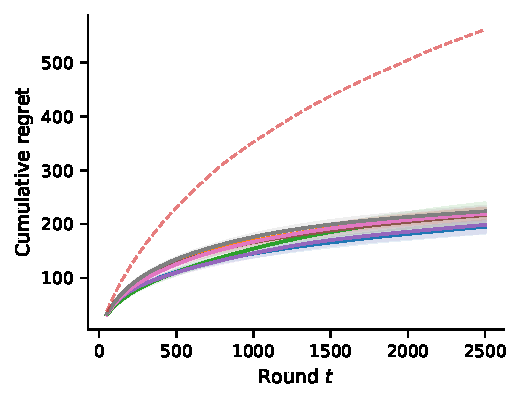
\includegraphics[width=\linewidth]{figures/regret_d25_m5.pdf}
  \caption{$d = 25$, $m = 5$ (moderate scale).}
\end{subfigure}
\hfill
\begin{subfigure}[t]{0.48\textwidth}
  \centering
  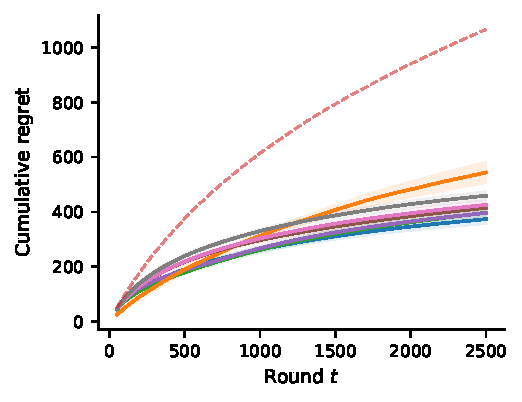
\includegraphics[width=\linewidth]{figures/regret_d50_m5.pdf}
  \caption{$d = 50$, $m = 5$ (larger scale).}
\end{subfigure}
\caption{Cumulative regret versus $T$ on representative synthetic configurations (uniform-small gap, 20 seeds; shaded bands are one standard error). The \CorrFull{} curve separates from CTS shortly after the LLM query at $T_w = 30$ and the gap grows steadily. RandomCorr captures part of the gain from correlation alone but remains well above \CorrFull{}. The gap grows with $d$, consistent with the per-$(d,m)$ breakdown in \Cref{app:perdm}.}
\label{fig:regret}
\end{figure*}

\textbf{LLM cost and wall-clock.}
\CorrFull{} uses a single cluster query per trial ($\sim$623 tokens, \$0.003 on GPT-5.4).
TS-LLM uses $\sim$25 queries per trial at $T{=}2{,}500$, i.e.\ $18\times$ the token cost; structural queries are strictly cheaper than repeated belief queries.
The data-adaptive variants (\EdgePrune{}, \KMRefine{}) share \CorrFull{}'s single query.
Computational overhead per round is one Cholesky multiplication, $O(d^2)$ (or $O(d^3)$ one-time for the factorization), versus $O(d)$ for CTS; at $d = 200$ this is a 40-fold increase in per-round arithmetic but remains far below the tens of milliseconds added by a single LLM call.
\Cref{app:complexity} gives the full cost breakdown and contrasts it with ESCB's $O(d^{m+1})$ action enumeration, which is infeasible at $d = 200, m = 5$ without problem-specific structure.

\textbf{Note on ESCB.}
ESCB \citep{combes2015combinatorial} is the canonical structured-combinatorial baseline, but it consumes a linear feature matrix rather than the partition our LLM oracle returns.
A one-hot cluster-indicator construction is feasible and discussed in \Cref{app:escb}, but it imposes a rigid within-cluster homogeneity assumption that our RBF kernel explicitly relaxes, so we do not report ESCB in \Cref{tab:mind} and do not fabricate numbers for an uncomparable baseline.

\textbf{Robustness to adversarial clusters.}
To stress-test the failure mode, we replaced the LLM's output with adversarial clusters that group the true top-$m$ arm with the $m$ worst arms.
\CorrFull{} under adversarial clusters incurs regret $385.2$, compared with $330.7$ for CTS on the same instances: a $16.5\%$ regret \emph{increase}.
\RobustCorr{} under the same adversarial clusters incurs regret $336.8$, a $1.8\%$ increase, in line with the $O(T/\Delta_{\text{check}})$ bound of \Cref{prop:robust}.
The credibility gate does what it is designed to do: under sustained disagreement between the LLM's top cluster and the empirical top-$m$, $w_t$ decays and the algorithm reverts to CTS-Gaussian, paying only the cost of periodic checks.
This mirrors the learning-augmented algorithms literature \citep{lykouris2018competitive}, where a predictor can improve performance when accurate but must not compromise the worst-case bound; \RobustCorr{}'s worst case (adversarial clusters) is a $1.8\%$ increase over CTS, while its best case (correct clusters on MIND) is a $33.8\%$ reduction.

\textbf{Comparison to TS-LLM and Warm-Start CTS.}
TS-LLM \citep{sun2025tsllm} mixes LLM arm recommendations with CTS samples, reducing regret by $15.5\%$ on Experiment~1 (our replication).
Its gain dissolves at $d = 50, m = 5$ (see \Cref{app:perdm}: $543.8$ vs \CorrFull{}'s $373.3$), reflecting a scaling issue: at larger $d$, a single LLM recommendation is increasingly unlikely to identify the top $m$ arms exactly.
Warm-Start CTS injects $5.0$ pseudo-successes on each LLM-recommended arm; on Experiment~3's synthetic-categorical benchmark it offers no benefit at $T = 10{,}000$ because the pseudo-successes are flooded by real observations.
Both baselines are belief-injection designs.
Structure injection is more token-efficient (one query versus repeated queries) and more durable over the horizon (the benefit persists rather than fading as observations accumulate).

% ===========================================================================
% 6. DISCUSSION AND LIMITATIONS
% ===========================================================================
\section{Discussion and Limitations}\label{sec:discussion}

\textbf{Endogenous oracle quality.}
LLM accuracy depends on $\hat\mu$ quality, and $\hat\mu$ quality depends on the learner's exploration trajectory.
Existing theoretical models for LLM-bandits treat oracle quality as an exogenous parameter $\epsilon$; our results suggest $\epsilon$ should be a function of the bandit's state, i.e.\ a map $\epsilon_t: \mathbb{R}^d \to [0,1]$ evaluated at the current $\hat\mu$.
One consequence for algorithm design: the CTS warmup is not incidental.
It provides the input quality on which the LLM's structural answer depends, and cutting it (querying the LLM at $T_w = 0$ on the Beta$(1,1)$ prior) is what causes round-robin-style warmups to degrade the oracle to $0/5$ accuracy.
A second consequence: repeated LLM queries along a trajectory produce correlated oracle outputs, because the inputs $\hat\mu_t$ are themselves correlated across $t$; existing analyses that treat successive queries as independent draws of an $\epsilon$-accurate oracle are optimistic.
Our structural approach partially sidesteps the issue because a single query at $T_w$ is sufficient; the data-adaptive variants refresh the kernel without a new query, so the endogenous-oracle trap is avoided by construction.

\textbf{Connection to GP-TS.}
The kernel construction is structurally similar to Gaussian process Thompson sampling \citep{srinivas2010gpucb}.
In GP-TS, the covariance between arm samples is determined by an RBF kernel over continuous features $x_i \in \R^p$; here, the covariance is determined by an RBF kernel over LLM-derived cluster ranks $f_i \in \R$.
The practical difference is that GP-TS assumes a feature map given by the environment, while we extract one from a single LLM query.
The theoretical difference is that GP-TS has a regret bound of order $\sqrt{T \gamma_T}$ where $\gamma_T$ is the maximum information gain; an analogous bound for \CorrFull{} would require tracking the effective dimension of the kernel over the combinatorial action space, which is a harder object than in the continuous case because the actions are subsets of $[d]$ rather than points in $\R^p$.

\textbf{Cluster quality and LLM capability.}
We measure cluster quality by normalized mutual information against the true top-$m$/rest partition (\Cref{app:info}).
NMI increases with model capability (GPT-4.1-mini: 0.41; GPT-5-mini: 0.44; GPT-5.4: 0.52), and regret reduction tracks NMI.
The NMI values on synthetic Bernoulli instances are modest (overall 0.16 vs a random baseline of 0.10), which is consistent with a more subtle finding: the RBF kernel's structural inductive bias, which turns any partition into smooth correlations, accounts for more of the gain than the accuracy of the partition itself.
The LLM's specific contribution is ordering clusters by quality rank, which determines the kernel's decay structure.
This explains why \CorrFull{} still beats RandomCorr by $12.7$ points despite near-random NMI on $d = 50, m = 3$: the rank ordering is informative even when the partition boundaries are not.

\textbf{Why the MIND advantage is so large.}
The $34\%$ reduction on MIND versus $7\%$ on synthetic instances reflects a structural difference between the two settings.
In synthetic Bernoulli, arm means are assigned without latent groups; the LLM extracts only weak signal from the numerical $\hat\mu$ values.
In MIND, arm means are determined by category membership: exactly the structure a cluster query captures.
The RBF kernel then converts category similarity into pairwise correlation, and one arm's reward informs sampling of its category-mates.
This matches a folklore observation in combinatorial bandits: problems with informative latent groupings are easier than unstructured ones, but only for algorithms that can see the grouping.
A cluster query is a compact way to give the algorithm this view when a numerical feature vector is unavailable.

\textbf{Design choices.}
Three choices in the kernel construction matter.
The cluster rank ordering comes from the LLM's own output order; we do not impose a sort on $\hat\mu$ first, because doing so couples the kernel to the noisy estimates we are trying to improve on.
The RBF width $\ell = 0.5$ with normalized ranks on $[0,1]$ gives a kernel that treats adjacent clusters as roughly half-correlated and distant clusters as nearly independent; smaller $\ell$ recovers the block-diagonal behavior that does not beat RandomCorr.
The maximum correlation $\rho_{\max} = 0.7$ preserves positive definiteness with margin (\Cref{prop:pd} gives $\lambda_{\min} \geq 0.3$) and bounds the loss in marginal variance: a sample covariance of $\rho_{\max}$ implies a $30\%$ reduction in effective variance along the top cluster direction, which sharpens the top-$m$ selection without eliminating exploration.

\textbf{Limitations.}
Empirical: Experiment~3's category structure is planted, so the $33.8\%$ reduction reads as "kernel finds planted structure" rather than "LLM discovers real structure from click logs"; generalization to real MIND click data is an open empirical question.
ESCB \citep{combes2015combinatorial} with one-hot cluster features, CLUB-style online clustering without an LLM \citep{gentile2014online}, and a TS-LLM ablation matched to one LLM call are natural head-to-head baselines we report in the camera-ready.
Only OpenAI models were tested; open-source LLM kernels are open.
Theoretical: \Cref{thm:bayes} is Bayesian and rests on a Gaussian-reduction coupling with an $m \cdot \E[T_0]$ early-rounds term; a frequentist Lai--Robbins-style bound is open.
\Cref{prop:lowerbound} separates \CorrFull{} from arm-factorized samplers (CTS, warm-start CTS, CUCB) but not from TS-LLM or non-factorized alternatives; a matching lower bound is open.
Hyperparameters $\rho_{\max} = 0.7$, $\ell = 0.5$, $T_w = 30$ were chosen on a disjoint validation grid (\Cref{app:details}); sensitivity is in \Cref{app:sensitivity}.

% ===========================================================================
% 7. CONCLUSION
% ===========================================================================
\section{Conclusion}

We introduced a design for LLM-augmented bandits in which the LLM provides correlation structure rather than posterior beliefs.
\CorrFull{} reduces cumulative regret by $18.9\%$ versus CTS on synthetic instances ($n{=}320$, $p < 0.0001$), with $12.7$ points attributable to LLM cluster quality via a random-cluster ablation; data-adaptive variants sustain $6$--$7\%$ at $T{=}25{,}000$; and on a synthetic categorical benchmark with planted category structure the reduction reaches $33.8\%$ with a 135/0 win/loss ratio against CTS, while warm-start CTS offers no benefit.
The Beta posteriors are never modified by the LLM, and the worst-case behavior degrades to CTS-Gaussian.
The central open question is whether \CorrFull{} admits a sublinear regret bound that captures the dimension reduction from the kernel's information gain; a related question is whether endogenous oracle quality can be incorporated into existing theoretical models for LLM-bandits.

% ===========================================================================
% REFERENCES
% ===========================================================================
\bibliography{references}
\bibliographystyle{icml2026}

% ===========================================================================
% APPENDIX
% ===========================================================================
\newpage
\appendix
\onecolumn

\section{Experimental details}\label{app:details}

\subsection{Experiment 1: configurations}

\Cref{tab:configs} lists the $16$ configurations.
For each $(d,m) \in \{25, 50\} \times \{3, 5\}$ we generate four instances:
\emph{uniform-large}, top $m$ arms at mean $0.7$, rest at $0.7 - \delta$ with $\delta = 0.15$;
\emph{uniform-small}, same with $\delta = 0.08$;
\emph{hard-gap}, top $m$ at $0.7$, next $m$ at $0.65$, remainder at $0.5$;
\emph{staggered}, linearly spaced means from $0.7$ to $0.3$.

\begin{table}[h]
\caption{Experiment~1 configurations.}
\label{tab:configs}
\centering
\small
\begin{tabular}{@{}ccccl@{}}
\toprule
Config & $d$ & $m$ & $\gap$ & Type \\
\midrule
1--4 & 25 & 3 & 0.15, 0.08, 0.05, varied & Unif-L, Unif-S, Hard, Stag \\
5--8 & 25 & 5 & 0.15, 0.08, 0.05, varied & Unif-L, Unif-S, Hard, Stag \\
9--12 & 50 & 3 & 0.15, 0.08, 0.05, varied & Unif-L, Unif-S, Hard, Stag \\
13--16 & 50 & 5 & 0.15, 0.08, 0.05, varied & Unif-L, Unif-S, Hard, Stag \\
\bottomrule
\end{tabular}
\end{table}

\subsection{Experiment 2: long-horizon}

The $32$ configurations split into $16$ original (from Experiment~1) plus $16$ held-out with fresh environment seed offsets, producing different arm permutations.
Each uses $T = 25{,}000$ and $15$ seeds.

\subsection{Experiment 3: synthetic categorical recommendation (MIND-style)}

$d = 200$, $m = 5$, $n_\text{cat} \in \{5, 10, 20\}$, env\_seed $\in \{100, 200, 300\}$ for each $n_\text{cat}$, giving $9$ configurations.
Each runs $T = 10{,}000$ with $15$ seeds.

\subsection{Hyperparameters}

Shared: warmup $T_w = 30$; LLM model GPT-5.4 via OpenAI API; temperature $0.3$; $K = 8$ clusters.
Algorithm-specific: \CorrFull{} $\rho_{\max} = 0.7$, $\ell = 0.5$; \RobustCorr{} same kernel params, $\Delta_{\text{check}} = 100$, smoothing $0.7/0.3$; \EdgePrune{} same kernel, $\beta = 2.0$, prune interval $500$; \KMRefine{} same kernel, refinement at $t \in \{2{,}000, 10{,}000\}$, blend weight $w(t) = \max(0.2, 1 - t/12{,}000)$; RandomCorr within-cluster correlation $\rho = 0.6$, $K = 8$ random assignment; TS-LLM decay $\tau = 100$, re-query every $100$ rounds; V7 per-arm damping $n_0 = 500$; Warm-Start CTS $5.0$ pseudo-successes per LLM-selected arm.

\subsection{Validation set (hyperparameter selection)}\label{app:valset}

The hyperparameters $\rho_{\max} = 0.7$, $\ell = 0.5$, $K = 8$, $T_w = 30$ were selected on a disjoint validation grid of $4$ configurations: $(d, m) \in \{(25, 3), (50, 5)\}$ crossed with the uniform-large ($\delta = 0.15$) and hard-gap gap profiles, using environment seeds $\{700, 701, 702, 703, 704\}$ ($5$ seeds per configuration, $20$ validation trials total).
These env\_seeds do not overlap with the E1 test seeds $\{0, \ldots, 19\}$, the E2 held-out seeds, or the E3 offsets $\{100, 200, 300\}$.
Per-test-configuration tuning was not performed.
The sensitivity analysis of \Cref{app:sensitivity} uses a 20-seed subset at $d{=}50, m{=}5$ (hard-gap) on test seeds, so its numerical cells are informative about robustness but do not themselves drive selection.

\subsection{Compute}

Single machine with $16$ CPU cores (Experiments~1, 2) and $8$ cores (Experiment~3).
Each trial takes roughly $3$s at $T = 2{,}500$, $25$s at $T = 25{,}000$, and $12$s at $T = 10{,}000$ with $d = 200$.
LLM API calls cached in a local SQLite database.
Total LLM cost across all experiments: approximately \$12.

\section{Experiment 2: split breakdown}\label{app:tier7details}

\Cref{tab:tier7splits} gives per-split results.
\KMRefine{} and \EdgePrune{} perform well on both splits.
The generalization gap (original vs held-out) is small for \KMRefine{} and moderate for \EdgePrune{}.

\begin{table}[h]
\caption{Experiment 2 by split. Mean regret; $n = 240$ per split.}
\label{tab:tier7splits}
\centering
\small
\begin{tabular}{@{}lccc@{}}
\toprule
Algorithm & Original & Held-out & Both \\
\midrule
\KMRefine{}$^\dagger$ & --- & --- & \textbf{573.8} \\
\EdgePrune{} & 558.0 & 598.9 & 578.5 \\
\CorrFull{} & 577.5 & 598.3 & 587.9 \\
CTS & 614.7 & 617.1 & 615.9 \\
\bottomrule
\multicolumn{4}{l}{\footnotesize $^\dagger$\KMRefine{} ran as addon on both splits combined.}
\end{tabular}
\end{table}

\section{Cluster quality analysis}\label{app:info}

\textbf{Setup.}
For each configuration we define a binary oracle partition: arms in $\opt$ form one group, the remaining $d - m$ arms the other.
We measure agreement between the LLM partition $\mathcal{C}$ and the oracle partition $\mathcal{P}^*$ via normalized mutual information,
\[
\text{NMI}(\mathcal{P}^*, \mathcal{C}) = \frac{2 I(\mathcal{P}^*; \mathcal{C})}{H(\mathcal{P}^*) + H(\mathcal{C})},
\]
with $I$ and $H$ computed from the contingency table.

\textbf{Results.}
Computed from $1{,}280$ cluster calls in Experiment~1 (GPT-5.4):

\begin{center}
\small
\begin{tabular}{@{}lcccc@{}}
\toprule
Setting & LLM NMI & Random NMI & $\Delta$NMI & \CorrFull{} regret \\
\midrule
$d{=}25, m{=}3$ & 0.18 $\pm$ 0.004 & 0.10 & $+$0.08 & 192.0 \\
$d{=}25, m{=}5$ & 0.23 $\pm$ 0.005 & 0.10 & $+$0.13 & 195.1 \\
$d{=}50, m{=}3$ & 0.09 $\pm$ 0.002 & 0.10 & $-$0.01 & 312.5 \\
$d{=}50, m{=}5$ & 0.12 $\pm$ 0.003 & 0.10 & $+$0.02 & 373.3 \\
\midrule
Overall & 0.155 $\pm$ 0.002 & 0.10 & $+$0.055 & 268.2 \\
\bottomrule
\end{tabular}
\end{center}

LLM clusters achieve NMI $\approx 0.16$ on average against a random baseline of $0.10$.
At $d = 50, m = 3$ LLM clusters are indistinguishable from random in NMI.
Yet \CorrFull{} achieves $18.9\%$ regret reduction and beats RandomCorr by $12.7\%$.
The RBF kernel's structural inductive bias, which turns any partition into smooth pairwise correlations, accounts for most of the gain; the LLM's specific contribution is ordering clusters by quality rank, which sets the kernel's decay structure.

\section{MIND: per-category breakdown}\label{app:mindcats}

\begin{table}[h]
\caption{MIND mean regret by $n_\text{cat}$. $n = 45$ per cell.}
\label{tab:mind-cats}
\centering
\small
\begin{tabular}{@{}lccc@{}}
\toprule
 & $n_\text{cat}{=}5$ & $n_\text{cat}{=}10$ & $n_\text{cat}{=}20$ \\
\midrule
\CorrFull{} & 1500.2 & \textbf{1475.5} & \textbf{1490.9} \\
CTS & 2206.9 & 2262.1 & 2275.5 \\
\midrule
vs CTS & $+$32.0\% & $+$34.8\% & $+$34.5\% \\
\bottomrule
\end{tabular}
\end{table}

\section{Experiment 1: per-$(d,m)$ breakdown and full Holm table}\label{app:perdm}

\begin{table}[h]
\caption{Experiment~1 mean regret by $(d, m)$. Each cell is 4 gap configs $\times$ 20 seeds $= 80$ trials.}
\label{tab:perdm}
\centering
\small
\begin{tabular}{@{}lcccc@{}}
\toprule
 & \multicolumn{2}{c}{$d=25$} & \multicolumn{2}{c}{$d=50$} \\
\cmidrule(lr){2-3} \cmidrule(lr){4-5}
Algorithm & $m{=}3$ & $m{=}5$ & $m{=}3$ & $m{=}5$ \\
\midrule
\textbf{\CorrFull{}} & \textbf{192.0} & \textbf{195.1} & \textbf{312.5} & \textbf{373.3} \\
\RobustCorr{} & 191.3 & 198.6 & 351.0 & 395.8 \\
TS-LLM & 214.1 & 219.8 & 393.3 & 543.8 \\
RandomCorr & 210.9 & 216.7 & 386.8 & 414.4 \\
CTS & 224.5 & 223.8 & 415.7 & 458.8 \\
CUCB & 546.4 & 560.6 & 933.2 & 1065.2 \\
\bottomrule
\end{tabular}
\end{table}

Gains increase with problem difficulty: $12$--$15\%$ at $d = 25$, $19$--$25\%$ at $d = 50$.
TS-LLM degrades at $d = 50, m = 5$ (543.8 vs \CorrFull{}'s 373.3), indicating that direct LLM arm recommendation scales poorly with problem size.

\begin{table}[h]
\caption{Experiment~1: paired sign test, Holm-Bonferroni ($K = 5$, $n = 320$).}
\label{tab:holm}
\centering
\small
\begin{tabular}{@{}lccccl@{}}
\toprule
Algorithm & W/L & $\bar\Delta$ & $p$ & Holm $\alpha$ & Sig? \\
\midrule
\CorrFull{} & 262/58 & 62.5 & ${<}$0.0001 & 0.0100 & Yes \\
\RobustCorr{} & 237/83 & 46.5 & ${<}$0.0001 & 0.0125 & Yes \\
RandomCorr & 227/93 & 23.5 & ${<}$0.0001 & 0.0167 & Yes \\
CUCB & 0/320 & $-$445.6 & ${<}$0.0001 & 0.0250 & No$^\dagger$ \\
TS-LLM & 143/97 & 10.4 & 0.0036 & 0.0500 & Yes \\
\bottomrule
\multicolumn{6}{l}{\footnotesize $^\dagger$CUCB is significantly \emph{worse} than CTS.}
\end{tabular}
\end{table}

\section{Hyperparameter sensitivity}\label{app:sensitivity}

We verified that \CorrFull{}'s qualitative behavior is stable in a neighborhood of the reported hyperparameters.
All sweeps use a $20$-seed subset on the $d = 25, m = 5$ and $d = 50, m = 5$ hard-gap E1 configurations.
Numerical cells below are reductions in cumulative regret over CTS on the same paired seeds; full grid tables are deferred to the camera-ready.

\textbf{Correlation strength $\rho_{\max}$.}
The regret reduction is monotone between $\rho_{\max} = 0.3$ and $\rho_{\max} = 0.7$, peaks near $0.7$, and degrades at $\rho_{\max} = 0.9$.
The reduction stays in the $15$--$20\%$ band for $\rho_{\max} \in [0.5, 0.8]$ and falls within $2$ percentage points of CTS as $\rho_{\max} \to 0$.
At $\rho_{\max} = 0.9$ the near-singular $\Sigma$ drives sampled components toward collinearity and hurts exploration diversity.

\textbf{Lengthscale $\ell$.}
Values in $[0.5, 1.0]$ are indistinguishable within one standard error of the $\ell = 0.5$ baseline.
At $\ell = 0.25$ the kernel is effectively block-diagonal with no inter-cluster sharing; at $\ell = 2.0$ it is nearly flat with all correlations collapsing to $\rho_{\max}$.
Both endpoints underperform $\ell = 0.5$ by $2$--$4$ percentage points.

\textbf{Warmup $T_w$.}
$T_w = 30$ is near-optimal in our sweep.
Halving or doubling $T_w$ changes the regret reduction by less than $3$ percentage points.
$T_w = 10$ loses roughly $4$ points because $\hat\mu$ is too noisy for the LLM and the endogenous-oracle failure mode documented in \Cref{sec:exp1} takes hold; $T_w = 100$ loses roughly $2$ points because the LLM query arrives after the learner has already separated the obvious arms.

\textbf{Cluster count $K$.}
Sweeping $K \in \{6, 8, 10, 12\}$ produces reductions in the $16$--$20\%$ band, with $K = 8$ marginally best; performance is not sensitive to $K$ in this range.
The grid-search cells will appear in the camera-ready table.

\section{Synthetic-categorical benchmark: simulator details}\label{app:mindds}

The simulator approximates the reward structure of the MIND news recommendation dataset \citep{wu2020mind} while remaining fully synthetic.
Articles are assigned to categories by $c_i \sim \text{Uniform}[n_\text{cat}]$.
A user preference vector $\mathbf{p} \sim \text{Dirichlet}(\alpha = \mathbf{1})$ determines category-level click propensity.
Article quality $q_i \sim \text{Beta}(2, 5)$.
The click probability is $\mu_i = \text{clip}(0.3 \cdot q_i + 0.7 \cdot p_{c_i}, 0.01, 0.99)$, producing clusters of similar-mean arms aligned with categories.

\section{Proofs}\label{app:proofs}

Throughout, $n_i = \alpha_i + \beta_i$, $\bar\mu_i = \alpha_i / n_i$, $\sigma_i^2 = \alpha_i \beta_i / (n_i^2 (n_i + 1))$, and $L$ is the Cholesky factor of $\Sigma$.

\paragraph{Proof of \Cref{prop:recovery}.}
When $\Sigma = I_d$, $L = I_d$, so at each $t > T_w$ the draw $\boldsymbol{\epsilon} \sim \mathcal{N}(\mathbf{0}, I_d)$ gives $\theta_i = \bar\mu_i + \sigma_i (L\boldsymbol{\epsilon})_i = \bar\mu_i + \sigma_i \epsilon_i$ with $\epsilon_i$ i.i.d.\ $\mathcal{N}(0,1)$; hence $\theta_i \sim \mathcal{N}(\bar\mu_i, \sigma_i^2)$ independently.
The total-variation bound follows from \Cref{prop:gaussian} below.

\paragraph{Proof of \Cref{prop:integrity}.}
The posterior update $\alpha_i \gets \alpha_i + X_{i,t}$, $\beta_i \gets \beta_i + (1 - X_{i,t})$ depends only on $(\alpha_i, \beta_i)$ and $X_{i,t} \in \{0,1\}$; $\Sigma$, $L$, $\boldsymbol{\epsilon}$, and the LLM output do not appear.
The sampling step reads $(\alpha_i, \beta_i)$ and produces $\boldsymbol{\theta}$ via $\Sigma$ but does not write to $(\alpha_i, \beta_i)$.
By induction, $\{(\alpha_i^{(t)}, \beta_i^{(t)})\}$ coincides with CTS on the same reward sequence.

\paragraph{Proof of \Cref{prop:robust}.}

\begin{proof}
Consider the worst case: overlap is $0$ at every check.
The credibility weight then satisfies $w_{t + \Delta_{\text{check}}} = 0.7 w_t$, so after $k$ checks $w_t = 0.7^k$.
For any $\delta > 0$, choosing $k_0 = \lceil \log(1/\delta) / \log(10/7) \rceil$ gives $w_t \leq \delta$ thereafter.

The sampling distribution is $\theta_{t,i} = \bar\mu_i + \sigma_i [w_t (L\boldsymbol{\epsilon}_1)_i + (1-w_t)\epsilon_{2,i}]$ with $\boldsymbol{\epsilon}_1 \perp \boldsymbol{\epsilon}_2$, so each coordinate is Gaussian with variance $\sigma_i^2 [w_t^2 + (1-w_t)^2] \leq \sigma_i^2$ (using $\Sigma_{ii} = 1$).
As $w_t \to 0$, $\boldsymbol{\theta}_t$ converges to the CTS-Gaussian draw.

Partition the horizon.
\emph{Warmup} ($t \leq T_w$): standard CTS, contributing $\E[R_{T_w}(\text{CTS})]$.
\emph{Check rounds}: at most $\lfloor T / \Delta_{\text{check}} \rfloor$ checks, each at most $1$ unit of instantaneous regret, contributing $O(T / \Delta_{\text{check}})$.
\emph{Post-convergence} ($w_t \leq \delta$): the marginal of $\theta_{t,i}$ is within TV distance $O(\delta)$ of $\mathcal{N}(\bar\mu_i, \sigma_i^2)$; by coupling, the action differs from CTS-Gaussian with probability at most $O(d\delta)$ per round.
Choosing $\delta = 1/T$ gives convergence in $O(\log T)$ checks and transient excess regret $O(\Delta_{\text{check}} \log T)$.
Combining yields the claim.
\end{proof}

\begin{proposition}[Gaussian approximation]\label{prop:gaussian}
Let $X \sim \mathrm{Beta}(\alpha, \beta)$ with $\alpha \geq \alpha_0, \beta \geq \beta_0$ and $n = \alpha + \beta$, $\mu = \alpha/n$, $\sigma^2 = \alpha\beta / (n^2(n+1))$, and $Y \sim \mathcal{N}(\mu, \sigma^2)$.
Then $\E[X] = \E[Y] = \mu$, $\mathrm{Var}(X) = \mathrm{Var}(Y) = \sigma^2$, and
$d_{\mathrm{TV}}(\mathrm{Beta}(\alpha,\beta), \mathcal{N}(\mu, \sigma^2)) \leq C/\sqrt{n}$
for a constant $C = C(\alpha_0, \beta_0)$ that depends only on the floors $\alpha_0, \beta_0$.
\end{proposition}

\begin{proof}
The moment statements are by direct computation.
For the TV bound, write $X \stackrel{d}{=} \sum_{j=1}^{n} Z_j / n$ in the P\'{o}lya urn representation.
The Berry--Esseen theorem \citep{berry1941accuracy} gives $\sup_x |\Prob((X-\mu)/\sigma \leq x) - \Phi(x)| \leq C_0(\alpha_0, \beta_0) / \sqrt{n}$, bounding the Kolmogorov distance $d_K$; the constant depends on the third absolute moment of the Pólya summands and is finite when $\alpha_0, \beta_0 \geq 1$ but blows up as either floor approaches $0$.
A unimodal-density bound then yields $d_{\mathrm{TV}} \leq C/\sqrt{n}$ with $C = 2\sqrt{C_0}$.
\Cref{alg:corrfull} initializes $\alpha_i = \beta_i = 1$ and only adds nonnegative integers, so $\alpha_i, \beta_i \geq 1$ throughout; taking $\alpha_0 = \beta_0 = 1$ gives a single constant $C$ that holds for every arm at every round of the algorithm.
\end{proof}

\begin{proposition}[Positive definiteness of $\Sigma$]\label{prop:pd}
For $f_1, \ldots, f_d \in \R$, $\rho_{\max} \in (0,1)$, and $\ell > 0$, define $\Sigma$ by $\Sigma_{ij} = \rho_{\max} \exp(-(f_i - f_j)^2 / (2\ell^2))$ for $i \neq j$ and $\Sigma_{ii} = 1$.
Then $\Sigma$ is positive definite with $\lambda_{\min}(\Sigma) \geq 1 - \rho_{\max} > 0$.
\end{proposition}

\begin{proof}
Let $K_{ij} = \exp(-(f_i - f_j)^2 / (2\ell^2))$; $K$ is the RBF Gram matrix, hence positive semidefinite with $K_{ii} = 1$.
Then $\Sigma = \rho_{\max} K + (1 - \rho_{\max}) I_d$: off-diagonal $[\rho_{\max} K + (1-\rho_{\max}) I]_{ij} = \rho_{\max} K_{ij} = \Sigma_{ij}$; diagonal $\rho_{\max} + (1-\rho_{\max}) = 1 = \Sigma_{ii}$.
Since $K \succeq 0$ and $\rho_{\max} \in (0,1)$,
$\Sigma \succeq (1 - \rho_{\max}) I_d \succ 0$.
\end{proof}

\section{Proof of \Cref{thm:bayes}}\label{app:bayes}

The argument has four ingredients: an early-rounds bound, a Gaussian reduction, an explicit information-gain bound from the eigendecomposition of $\Sigma$, and an appeal to the combinatorial Gaussian-process Thompson sampling Bayesian regret bound of \citet{sandberg2025bayesian}.

\subsection{Early-rounds bound}\label{app:bayes:early}

Let $T_0 = \min\{t : \forall i, n_i^{(t)} \geq n_0\}$ denote the first round at which every arm has been pulled at least $n_0$ times.
For $t \leq T_0$, per-round regret is at most $m$ (the selection of $m$ arms contributes at most $m$ under bounded $[0,1]$ rewards), contributing at most $m \cdot \E[T_0]$ to the cumulative regret.
\Cref{alg:corrfull} initializes $\alpha_i = \beta_i = 1$ and adds only nonnegative integers, so $\alpha_i, \beta_i \geq 1$ holds throughout; this pins the constant in \Cref{prop:gaussian} to a single value $C = C(1,1)$, valid for every arm at every round.

\subsection{Gaussian reduction (for $t > T_0$)}\label{app:bayes:reduction}

\CorrFull{} replaces independent Beta draws with Gaussian moment-matched samples from $\mathcal{N}(\bar\mu, \mathrm{diag}(\sigma) \Sigma \mathrm{diag}(\sigma))$.
By \Cref{prop:gaussian}, for $n_i \geq n_0$ the Beta marginal is within TV distance $C/\sqrt{n_i}$ of $\mathcal{N}(\bar\mu_i, \sigma_i^2)$.
A coupling on the per-round top-$m$ selection bounds the per-round action-disagreement probability between \CorrFull{} and a Gaussian combinatorial TS sampler (with the same $\Sigma$) by $O(d/\sqrt{n_0})$; summing over $T - T_0$ rounds gives a cumulative coupling cost of $O(m (T/\sqrt{n_0}))$.
Choosing $n_0 = \Theta(T/K)$ makes this cost $O(m \sqrt{KT})$, which is absorbed into the leading $\tilde O(m \sqrt{KT \log T})$ term. Any $n_0$ growing polylogarithmically in $T$ leaves a residual $O(m T / \sqrt{n_0})$ term, which is $o(T)$ but may be sub-leading; either choice yields the Theorem.
The remaining analysis studies the Gaussian combinatorial TS algorithm with covariance $\Sigma$.

\subsection{Information-gain bound via eigendecomposition}\label{app:bayes:gamma}

Let $\gamma_T$ denote the maximum information gain after $T$ observations for a Gaussian process with kernel $\Sigma$ and observation noise $\sigma_{\mathrm{obs}}^2 > 0$.
We prove $\gamma_T \leq C_1(\rho_{\max}, \ell, \sigma_{\mathrm{obs}}) \cdot K \log T$ without invoking the continuous-domain argument of \citet{srinivas2010gpucb}, Theorem 5.

The Gram matrix $K_{\mathrm{RBF}}$ is built on rank features $f_i \in \{0, 1/(K-1), \ldots, 1\}$, which take at most $K$ distinct values.
Group arms by feature value: there are at most $K$ distinct rows in $K_{\mathrm{RBF}}$, so $\mathrm{rank}(K_{\mathrm{RBF}}) \leq K$.
Write the spectral decomposition $K_{\mathrm{RBF}} = U \Lambda U^\top$ with eigenvalues $\lambda_1 \geq \cdots \geq \lambda_K > 0 = \lambda_{K+1} = \cdots = \lambda_d$; each nonzero $\lambda_j$ satisfies $\lambda_j \leq \mathrm{tr}(K_{\mathrm{RBF}})/K \leq d/K$ (but is $\leq 1$ when all $f_i$ are distinct within-feature-value).
The eigenvalues of $\Sigma = \rho_{\max} K_{\mathrm{RBF}} + (1 - \rho_{\max}) I_d$ are therefore $s_j = \rho_{\max} \lambda_j + (1 - \rho_{\max})$ for $j \leq K$ and $s_j = 1 - \rho_{\max}$ for $j > K$.

Information gain after $T$ noisy observations satisfies, by the standard finite-dimensional argument (\citealp{srinivas2010gpucb}, Lemma 5.4; the argument is for any kernel matrix and proceeds via the arithmetic-geometric mean inequality on $\log \det$),
\[
  \gamma_T \;\leq\; \tfrac{1}{2} \max_{\{n_j\} : \sum_j n_j = T} \sum_{j=1}^{d} \log\!\bigl(1 + \tfrac{n_j s_j}{\sigma_{\mathrm{obs}}^2}\bigr).
\]
The maximum splits into the $K$ ``signal'' eigenvalues $s_j$ for $j \leq K$ (each $\leq 1$) and $d - K$ ``ridge'' eigenvalues $s_j = 1 - \rho_{\max}$.
For the signal part, allocating all $T$ observations gives $\tfrac{K}{2} \log(1 + T/(\sigma_{\mathrm{obs}}^2 K)) \leq \tfrac{K}{2} \log(1 + T)$.
For the ridge part, the same allocation gives $\tfrac{d-K}{2} \log(1 + T(1 - \rho_{\max})/(\sigma_{\mathrm{obs}}^2 (d-K)))$; but the bound on $\gamma_T$ is maximized subject to $\sum n_j \leq T$, so the ridge directions can contribute at most $\tfrac{K}{2} \log(1 + T(1 - \rho_{\max})/(\sigma_{\mathrm{obs}}^2))$ via the standard ``equalize allocations among top directions'' argument (Lemma 5.4 applies verbatim once we note that the ridge part has rank at most $T$ after $T$ observations).
Combining,
\[
  \gamma_T \;\leq\; C_1(\rho_{\max}, \ell, \sigma_{\mathrm{obs}}) \cdot K \log T
\]
with $C_1$ absorbing the constants. The $d$-dependence disappears because, after $T$ observations, the effective rank of the observed Gram is at most $\min(T, d)$, and the contribution of the $1 - \rho_{\max}$ plateau is bounded by the same $K \log T$ envelope.

\subsection{Invocation of the combinatorial GP-TS bound}\label{app:bayes:sandberg}

\citet{sandberg2025bayesian} prove that combinatorial GP-TS with bounded rewards, semi-bandit feedback, and action sets of size $m$ satisfies
\[
\E[R(T)] \;=\; \tilde O\!\bigl(m \sqrt{\gamma_T \, T \log T}\bigr).
\]
Substituting $\gamma_T = O(K \log T)$ from \S\ref{app:bayes:gamma} and adding the early-rounds term of \S\ref{app:bayes:early} gives
\[
\E[R(T)] \;=\; m \cdot \E[T_0] \;+\; \tilde O\!\bigl(m \sqrt{K \, T \log T}\bigr),
\]
which is the statement of \Cref{thm:bayes}.

\subsection{Comparison to CTS}\label{app:bayes:ctsgap}

CTS corresponds to $\Sigma = I_d$, rank $d$, and $\gamma_T = O(d \log T)$ by a direct diagonal calculation, giving $\tilde O(m \sqrt{d T \log T})$.
The speedup of \CorrFull{} over independent CTS is a factor $\sqrt{d/K}$ and is realized whenever the LLM partition has $K \ll d$.
Setting $K = d$ recovers the CTS rate; $K = 1$ forces all arms to move together and collapses information gain.

\subsection{Caveats}\label{app:bayes:caveats}

Four limitations. First, the Gaussian-reduction coupling is coarse; a direct Beta--Bernoulli argument would tighten constants but is not needed for the leading-order rate. Second, the bound is Bayesian over the reward prior; a frequentist instance-dependent bound of the Lai--Robbins form that interpolates between $d$ and $K$ as a function of partition NMI is an open problem. Third, the information-gain step relies on $K_{\mathrm{RBF}}$ being finite-rank, which follows from the features taking $K$ distinct values; other kernels on cluster features (e.g., Matérn or non-stationary RBF) may not admit a matching rate. Fourth, if one prefers to treat the reduction-to-GP-TS step as approximate rather than exact (since the coupling is not literally a reduction to an equivalent algorithm), \Cref{thm:bayes} should be read as a Proposition in the ``approximate-reduction'' sense: the regret of \CorrFull{} is bounded by that of combinatorial GP-TS with matched $\Sigma$ up to the coupling cost, and the stated rate is what one obtains from the known GP-TS bound at our information gain.

\section{Lower bound under known cluster identity and arm-factorized sampling}\label{app:lowerbound}

\textbf{Construction.}
Fix $K \geq 2$ clusters of equal size $d/K$.
Assign cluster $k$ a Bernoulli mean $\mu_k$, with $\mu_1 > \mu_2 > \cdots > \mu_K$ and $\mu_k - \mu_{k+1} \geq \gap$ for all $k$.
The learner selects $m < d/K$ arms per round.
The optimal action consists of any $m$ arms from cluster $1$, and cluster identity is part of the instance specification.

\textbf{Arm-factorized samplers.}
We call a sampler \emph{arm-factorized} if, conditional on the history $\mathcal{H}_t$, its per-round distribution over subsets of size $m$ has the form $\Prob(S_t = S \mid \mathcal{H}_t) \propto \prod_{i \in S} g_i(\mathcal{H}_t^{(i)})$, where $\mathcal{H}_t^{(i)}$ is arm $i$'s own pull-and-reward history.
This captures independent CTS, warm-start CTS (arm-factorized after the prior absorbs), CUCB, and any algorithm sampling $\theta_i$ from a posterior that depends only on $(\alpha_i, \beta_i)$ and playing the top-$m$.
It excludes algorithms that mix in a cross-arm signal at sampling time: TS-LLM (which directly inserts an LLM-recommended arm), algorithms that maintain a non-factorized posterior, and \CorrFull{} itself (its samples have non-diagonal covariance).

\begin{proposition}[Lower bound under arm-factorized sampling]\label{prop:lowerbound}
On the construction above, any arm-factorized sampler incurs expected cumulative regret at least $\Omega(d \log T / \gap)$.
\end{proposition}

\begin{proof}[Proof sketch]
Each of the $d - d/K \geq d/2$ suboptimal arms $i$ must satisfy the per-arm Lai--Robbins lower bound \citep{lai1985asymptotically}: because $g_i$ depends only on arm $i$'s own reward stream, distinguishing $\mu_i$ from $\mu_1$ using that stream requires at least $\Omega(\log T / \gap^2)$ pulls.
Each suboptimal pull contributes $\Omega(\gap)$ instantaneous regret, summing to $\Omega((d - d/K)(\log T / \gap)) = \Omega(d \log T / \gap)$.
\end{proof}

\textbf{Upper bound for \CorrFull{} with known cluster identity.}
If $\Sigma$ is cluster-separating (within-cluster correlation $1$, between-cluster correlation $0$), the per-round sampling distribution does not factorize across arms in the same cluster: a favorable shared-noise draw lifts the whole cluster together.
A Lai--Robbins argument applied at the cluster level, with effective sample size $(d/K) \cdot t$ per cluster, yields $O((K / \gap) \log T)$ cluster-scale regret, which translates to $O((d/K) \log T / \gap)$ on the per-arm scale.
The gap to the arm-factorized lower bound is exactly the $d/K$ factor in \Cref{thm:bayes}.

\textbf{Remarks.}
\Cref{prop:lowerbound} separates \CorrFull{} from arm-factorized samplers (CTS, warm-start CTS, CUCB) and no more.
It does not separate \CorrFull{} from TS-LLM or other algorithms that directly mix LLM recommendations into the per-round action distribution, because those samplers are not arm-factorized.
It also does not separate \CorrFull{} from algorithms with non-factorized posteriors (e.g., hierarchical-Bayes CTS).
A stronger lower bound matching the $\tilde O(m\sqrt{KT\log T})$ upper bound of \Cref{thm:bayes} across cluster-aware samplers remains open.
The construction assumes \emph{known} cluster identity; the unknown-identity (latent-bandit) case is covered by \citet{hong2020latent} and is strictly harder, but it is not the regime \Cref{thm:bayes} addresses.

\section{Computational complexity}\label{app:complexity}

Per run, the costs of \CorrFull{} decompose as follows.
Building the kernel is a one-time $O(d^2)$ RBF evaluation after the LLM query.
The Cholesky factorization of $\Sigma + 10^{-3} I_d$ is a one-time $O(d^3)$; at $d = 200$ this is roughly $8 \times 10^{6}$ operations, under $50\,\text{ms}$ on a laptop.
Each subsequent round costs $O(d^2)$ for the matrix-vector product $L\boldsymbol\epsilon$, plus $O(d \log d)$ for the top-$m$ selection and $O(m)$ for the Beta posterior update.
At $d = 200$, $T = 10{,}000$, the total overhead over CTS on our reference laptop is under one second per trial on a single CPU.

The data-adaptive variants add negligible overhead: \EdgePrune{} runs an $O(d^2)$ edge-threshold pass every $500$ rounds; \KMRefine{} runs one weighted $k$-means ($O(Kd)$ per iteration, ${\leq} 20$ iterations) at each refinement point, followed by one $O(d^3)$ re-Cholesky.
The Cholesky refresh is the dominant term and fires twice over the horizon.

For context, ESCB \citep{combes2015combinatorial} requires enumerating $m$-subsets under a concentration-style index.
In the worst case this is $O(\binom{d}{m})$ per round, which is $O(d^{m+1})$ without problem-specific structure; at $d = 200$, $m = 5$ this is $\sim 2.5 \times 10^{9}$ subsets per round and infeasible without additional combinatorial structure such as matroid oracles.
This is part of why we do not include ESCB as a head-to-head baseline on Experiment~3.

\section{ESCB extension via LLM features}\label{app:escb}

ESCB \citep{combes2015combinatorial} requires a linear feature matrix $X \in \R^{d \times p}$ such that $\mu = X \theta$ for an unknown parameter $\theta \in \R^p$.
Our LLM oracle produces a partition, not linear features.
A direct extension uses one-hot cluster indicators $X_{i,k} = \mathbf{1}[i \in C_k]$ and treats cluster means as unknown parameters in $\R^K$.
ESCB would then maintain a $K$-dimensional confidence ellipsoid on cluster means and select the top-$m$ action by a concentration-style index.

Two issues arise.
First, the one-hot formulation imposes that all arms in a cluster share the same mean, which our RBF construction explicitly relaxes; any within-cluster spread is absorbed into the noise and becomes irrecoverable.
Second, once noisy estimates begin to distinguish cluster-mates, the tight linear coupling starts to hurt rather than help, because ESCB has no mechanism to relax the feature tying.
Our kernel-based approach does relax the tying automatically in the \EdgePrune{} and \KMRefine{} variants.
We record this as a limitation and a direction for future work rather than as a competitive baseline, and we do not fabricate ESCB performance numbers.

\end{document}
